\documentclass[10pt]{article}
\usepackage[preprint]{tmlr}
\usepackage{hyperref,url,booktabs,graphicx,amsmath,xcolor,microtype}
\usepackage{tikz}
\usetikzlibrary{positioning,arrows.meta,shapes.geometric}

\title{A 149M Text Encoder as the First Tier for Phone Agents:\\Pre-Registered Routing to Frontier Models}

\author{\name Chaitanya Talapalli \email chayt128@gmail.com\\
\addr Independent researcher}

\def\month{10}
\def\year{2026}
\def\openreview{}

\newcommand{\pts}{\,pts}

\begin{document}
\maketitle

\begin{abstract}
Phone agents usually send every step to a frontier language model, although many steps are easy. We test whether a 149M-parameter model that reads the screen's accessibility tree can answer the steps it is confident about and pass the rest to a frontier model, offline and with a human-written instruction for each step. Each registered hypothesis, with its threshold and sample, was fixed in a dated log before any frontier model saw its steps; analyses that were not registered are marked as such. On AndroidControl the small model answers 71--75\% of steps on the device, and routing the rest to Claude Opus~5.5, given 16 retrieved training examples, was non-inferior to Opus alone in every registered comparison at under a third of its cost. Pooled over the 1{,}650 test steps not used to set its threshold, routing is more accurate than Opus alone by 1.5 points ($[+0.5, +2.4]$, $p=0.006$; 1.1 points on corrected labels), although the small model alone is not; the gain comes from the two models erring on different steps. With Claude Sonnet~5.5 as the fallback, routing lifts Sonnet by 2.4--2.7 points ($p<0.001$) and also scores above the small model alone in both runs. A retrain that never used the test split reproduces the small model's accuracy, and under the protocol used by screenshot agents the text-only model scores 86.1\% on AndroidControl-Low, above the 85.2\% reported for OS-Atlas-7B on a slightly different step set. In a further registered test on 1{,}000 fresh in-domain steps, with Claude Haiku~5.5 as the fallback, showing the fallback only the small model's five best elements was as accurate as showing the whole screen at half the input. The evidence covers single steps only: a related cascade lost to a frontier agent on live multi-step tasks. We release the model, per-step outputs of every system and the registration log.
\end{abstract}

\section{Introduction}
A phone agent reads the screen, chooses an action, acts, and repeats. The most accurate agents call a frontier model at every step, which costs money, adds a network round trip and sends the screen's contents off the device. Many steps are nevertheless easy: tap the tab labelled ``Timers'', press ``5'', go back. If a small local model answered those steps and deferred only the hard ones, most frontier calls would disappear.

Deferring uncertain inputs to a stronger decision maker is well studied in selective classification~\citep{chow,geifman} and learning to defer~\citep{mozannar}, and routing between cheap and expensive language models is an active area~\citep{frugalgpt,automix,hybridllm,routellm}. Phone agents have recently adopted the idea: OpenPhone~\citep{openphone}, MAI-UI~\citep{maiui} and CORE~\citep{core} combine a billion-parameter local model with a cloud model and report end-to-end gains. Two questions remain open. How much of a phone agent's work can a model one to two orders of magnitude smaller take on, step by step, without costing the frontier model accuracy? And is the comparison fair? Small fine-tuned models are routinely compared with frontier models prompted zero-shot~\citep{limac}, a known source of inflated gains~\citep{melis,dacrema}.

We answer both questions on AndroidControl~\citep{androidcontrol} under a pre-registered protocol (Fig.~\ref{fig:overview}). Our contributions are:
\begin{itemize}\setlength\itemsep{1pt}
\item A routing study on 1{,}000 held-out steps with three frontier models (Opus and Sonnet each run twice), broken down by unseen apps and action types, and re-scored on corrected labels, plus a registered test on 650 further steps in which routing is significantly more accurate than the frontier model alone, with either of two deferral rules (Sec.~\ref{sec:router}).
\item A clean retrain that never used the test split, and a fair-baseline study showing that the small model's 6--8 point lead over zero-shot frontier models disappears once those models see similar solved examples (Sec.~\ref{sec:fair}).
\item A registered test of a fallback that sees only the small model's top five elements instead of the whole screen (Sec.~\ref{sec:sl}).
\item On-device measurements on a phone CPU, a quantized model evaluated end to end, a live phone demonstration, and a live multi-step result that bounds the claims (Secs.~\ref{sec:device} and~\ref{sec:live}).
\item The released model, per-step outputs of every system and the registration log (Appendix~\ref{app:reg}).
\end{itemize}
The model design follows candidate selection in MindAct~\citep{mind2web} and LiMAC~\citep{limac}, and the learned rule is a plain two-estimator form of learning to defer~\citep{mozannar}. What is new is the evidence: a model one to two orders of magnitude smaller than the billion-parameter local tiers above can serve as the first tier, a router that weighs the small model's chance of being right against the frontier model's beats the frontier model alone on registered fresh data, and the comparison holds against a frontier baseline given the same in-domain data.

\begin{figure}[t]
\centering
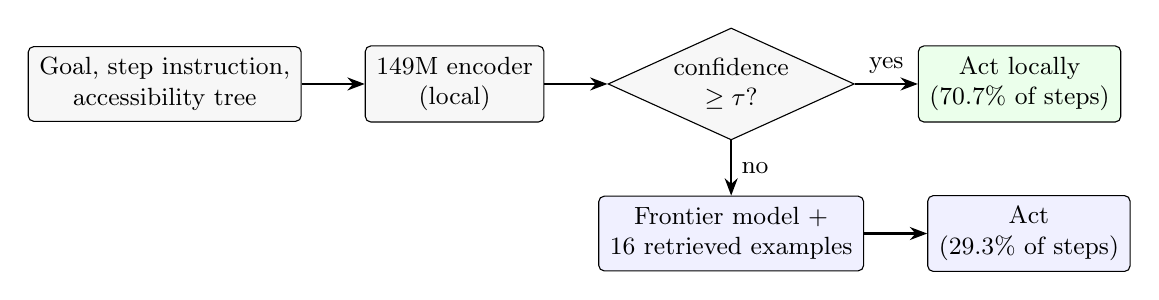
\begin{tikzpicture}[font=\small, node distance=6mm and 8mm,
  box/.style={draw, rounded corners=2pt, align=center, minimum height=9mm, inner sep=4pt, fill=gray!6},
  dec/.style={draw, diamond, aspect=2.2, align=center, inner sep=1pt, fill=gray!6},
  arr/.style={-{Stealth[length=2.2mm]}, thick}]
\node[box] (in) {Goal, step instruction,\\accessibility tree};
\node[box, right=of in] (enc) {149M encoder\\(local)};
\node[dec, right=of enc] (gate) {confidence\\$\geq\tau$?};
\node[box, right=of gate, fill=green!8] (local) {Act locally\\(70.7\% of steps)};
\node[box, below=7mm of gate, fill=blue!6] (cloud) {Frontier model +\\16 retrieved examples};
\node[box, right=of cloud, fill=blue!6] (act2) {Act\\(29.3\% of steps)};
\draw[arr] (in) -- (enc); \draw[arr] (enc) -- (gate);
\draw[arr] (gate) -- node[above]{yes} (local);
\draw[arr] (gate) -- node[right]{no} (cloud);
\draw[arr] (cloud) -- (act2);
\end{tikzpicture}
\caption{Local-first routing. The small model predicts an action and a confidence; steps at or above the threshold $\tau$ are answered locally, the rest by a frontier model shown similar solved examples. The threshold was fixed before the evaluation.}\label{fig:overview}
\end{figure}

\section{Related Work}
\paragraph{Phone and GUI agents.} AndroidControl~\citep{androidcontrol} provides step-level supervision with out-of-distribution splits; AndroidControl-Curated~\citep{accurated} corrects its labels. Screenshot agents such as OS-Atlas~\citep{osatlas}, UI-TARS~\citep{uitars}, InfiGUI-R1~\citep{infiguir1} and Ferret-UI Lite~\citep{ferretlite} lead the benchmark. LiMAC~\citep{limac} is the closest small system. AndroidWorld~\citep{androidworld} evaluates agents live. AutoDroid-V2~\citep{autodroidv2} lets a small on-device model write multi-step scripts instead of choosing one action at a time.

\paragraph{Deferral and routing.} Selective classification abstains at low confidence~\citep{chow,geifman}, and learning to defer trains a model to hand cases to an expert~\citep{mozannar}. For language models, FrugalGPT~\citep{frugalgpt} cascades APIs from cheap to expensive, AutoMix~\citep{automix} escalates after self-verification, and Hybrid LLM~\citep{hybridllm} and RouteLLM~\citep{routellm} learn routers. For phone agents, OpenPhone~\citep{openphone} escalates hard subtasks from a 3B on-device model to the cloud, MAI-UI~\citep{maiui} hands off when the local trajectory drifts from the user's intent and reports over 40\% fewer cloud calls, and CORE~\citep{core} lets a local model rank screen regions so that the cloud model sees less of the screen. Our local model is far smaller, and we isolate its effect at the step level against a frontier baseline matched for in-domain data.

\paragraph{Fair baselines.} Retrieved demonstrations raise frontier models' mobile-agent accuracy substantially~\citep{learnact,raggui}; we use retrieval only to strengthen the baseline. Under-tuned baselines have inflated reported gains across machine learning~\citep{melis,dacrema,musgrave,lipton}, and model accuracy depends on prompt format~\citep{sclar}, element order~\citep{ordering} and reasoning budget~\citep{inversettc}. Computer-use agents vary across reruns~\citep{cuareliability,beyondpass}, which motivates our replication.

\section{Method}\label{sec:method}
\paragraph{Task.} Each AndroidControl step provides the task goal, a human-written instruction for the step and the accessibility tree of the current screen. The system outputs one of 11 actions (tap, long press, type text, scroll in one of four directions, back, home, open app, wait) with its argument. Evaluation is offline: every step starts from the recorded history.

\paragraph{Small model.} Each accessibility tree is flattened into at most 220 elements, each rendered as class, visible text or description, hint, resource-id words, a coarse screen position and state flags. A ModernBERT-base encoder~\citep{modernbert} (149M parameters) reads the instruction, a one-line history (previous action and whether the screen changed) and the goal, followed by the elements, each preceded by a marker token. Three heads predict the action type, the target element (one logit per marker) and, for typed text and app names, a span copied from the instruction. We release the model as Milo Pointer. Training details and a preliminary comparison with generative models are in Appendix~\ref{app:train}.

\paragraph{Routing.} Confidence is the probability of the predicted action type, multiplied for taps by the probability of the chosen element. A step is answered locally if its confidence is at least $\tau = 0.9854$, the 30th percentile on a separate sample of 1{,}000 test steps; $\tau$ was fixed before any frontier model saw the evaluation steps.

\paragraph{Frontier baseline.} Claude Opus~5.5, Sonnet~5.5 and Haiku~5.5 (API identifiers \texttt{claude-opus-5-5}, \texttt{claude-sonnet-5-5}, \texttt{claude-haiku-5-5}; Claude Fable~5.1, \texttt{claude-fable-5-1}, a higher-priced Anthropic model, appears in Sec.~\ref{sec:fair}) receive a system prompt describing the actions and stating the dataset's conventions (scroll direction is named by where new content comes from, so a finger swipe up is a scroll down; wait when the last action has not taken effect), the same inputs as the small model, and 16 solved training steps retrieved by TF-IDF similarity of goal and instruction, each with its correct action and, for taps, the target element in words. The routing arms use adaptive reasoning at medium effort through the Batch API; the earlier arms in Table~\ref{tab:frontier} list their effort. We call this setting few-shot (FS). The baseline is thus retrieval-augmented: on AndroidControl's templated tasks the retrieved examples are often close to the test step, and its cost includes the 16 examples. This is deliberate, so that both tiers draw on the same in-domain data; measured against zero-shot Opus instead, the routed system costs about half as much.

\paragraph{Metric, statistics and costs.} A step is correct if the action type matches the record and, for taps, the centre of the chosen element lies inside the recorded target; typed text must match exactly after normalisation. We report paired differences with Wald 95\% intervals and exact McNemar tests; intervals computed by resampling whole episodes are essentially identical. The registered non-inferiority margin is 2 points, about a quarter of the gain Opus gets from examples (7.9 points); because a per-step loss compounds over a task, it suits single-step claims only. Costs are billed tokens at October 2026 Batch API prices (per million input/output tokens before the 50\% batch discount: Fable \$10/\$50, Opus \$4/\$20, Sonnet \$2/\$10, Haiku \$0.10/\$0.50, so Fable costs about 2.5 times Opus at similar token counts); real-time prices double every figure without changing ratios. On-device compute is not priced.

\paragraph{Pre-registration.} Each comparison was written to a dated log, with hypotheses, sample, threshold and margin, and committed to version control before any frontier request on its data. The log is self-hosted rather than held by a third-party registry. As an external check, every frontier run was submitted through the Message Batches API, which records the batch creation time on the provider's servers; for every routing study the registration commit precedes its batch (released table of commits and batch identifiers).

\paragraph{Samples and the test split.} AndroidControl has no validation split, and the original model's design was chosen while comparing variants on the test split; every number below comes from that model unless a clean retrain is named (Secs.~\ref{sec:fair} and~\ref{sec:sl}, and the pruned-input retrain in Sec.~\ref{sec:device}). A retrain whose every choice used a validation split carved from training reaches the same accuracy (Sec.~\ref{sec:fair}). Table~\ref{tab:design} lists the samples and what each was used for.

\begin{table}[t]\centering\small
\caption{Evaluation samples. The first three are disjoint samples of the AndroidControl test split.}\label{tab:design}
\begin{tabular}{lrp{0.58\linewidth}}\toprule
Sample & Steps & Used for\\\midrule
Calibration sample & 1{,}000 & Setting $\tau$; fitting the learned rule; fair-baseline study (Sec.~\ref{sec:fair})\\
Held-out sample & 1{,}000 & Registered routing tests, two runs; setting the learned rule's threshold\\
Confirmatory sample & 650 & Registered test of both frozen rules; drawn from 247 test episodes in no earlier sample\\
Shortlist sample & 1{,}000 & Registered shortlist test (Sec.~\ref{sec:sl}); validation episodes of the clean retrain\\
Full test split & 8{,}444 & Small-model accuracy, clean retrains, curated labels\\
Strict app holdout & -- & Small model retrained without 72 apps; tested on their 1{,}246 training-split episodes\\\bottomrule
\end{tabular}\end{table}

\section{Local-First Routing}\label{sec:router}
The evaluation set is 1{,}000 test steps (579 episodes) drawn at random from the 836 test episodes not used to set $\tau$. We registered that routing to Opus is non-inferior to Opus alone; that at least 60\% of steps stay local; and that routing to Sonnet is non-inferior both to Sonnet alone and to Opus alone. Routing to Haiku was registered later, after an internal review.

\begin{table}[t]\centering\small
\caption{Correct steps out of 1{,}000 held-out steps. Run 2 repeats every frontier request unchanged. Cost per 1{,}000 steps from billed tokens (Batch API).}\label{tab:router}
\begin{tabular}{lrrrr}\toprule
System & Run 1 & Run 2 & Answered locally & Cost (\$)\\\midrule
Small model alone & 869 & 869 & 100\% & 0\\\midrule
Opus 5.5 FS alone & 882 & 879 & 0\% & 9.54\\
Small model $\rightarrow$ Opus 5.5 FS & \textbf{892} & \textbf{890} & 70.7\% & 2.82\\\midrule
Sonnet 5.5 FS alone & 857 & 862 & 0\% & 4.80\\
Small model $\rightarrow$ Sonnet 5.5 FS & \textbf{881} & \textbf{889} & 70.7\% & 1.41\\\midrule
Haiku 5.5 FS alone & 805 & -- & 0\% & 0.26\\
Small model $\rightarrow$ Haiku 5.5 FS & 865 & -- & 70.7\% & $\approx$0.08\\\bottomrule
\end{tabular}\end{table}

\begin{table}[t]\centering\small
\caption{Paired differences in points, with 95\% CI and exact McNemar $p$. Last column: registered hypothesis and outcome.}\label{tab:diffs}
\begin{tabular}{llll}\toprule
Comparison & Run 1 & Run 2 & Registered\\\midrule
Small$\rightarrow$Opus vs Opus alone & $+1.0$ $[-0.2,+2.2]$, $p{=}0.14$ & $+1.1$ $[-0.2,+2.4]$ & non-inferior: held\\
Small$\rightarrow$Sonnet vs Sonnet alone & $+2.4$ $[+1.1,+3.7]$, $p{=}0.0005$ & $+2.7$ $[+1.3,+4.1]$ & non-inferior: held\\
Small$\rightarrow$Sonnet vs Opus alone & $-0.1$ $[-1.7,+1.5]$ & $+1.0$ $[-0.7,+2.7]$ & non-inferior: held\\
Small$\rightarrow$Haiku vs Opus alone & $-1.7$ $[-3.5,+0.1]$ & -- & non-inferior: failed\\
Small$\rightarrow$Opus vs small alone & $+2.3$, $p{=}0.011$ & & --\\
Small alone vs Opus alone & $-1.3$ $[-3.4,+0.8]$ & & --\\\bottomrule
\end{tabular}\end{table}

\paragraph{Results.} The small model answers 70.7\% of steps (Table~\ref{tab:router}). Routing to Opus scores 892 against 882 for Opus alone: non-inferior, not significantly better. Routing to Sonnet lifts Sonnet by 2.4 points and reaches Opus alone; the routed system (881 and 889 in the two runs) also scores above the small model alone (869; $+1.2$, $p=0.20$, and $+2.0$, $p=0.03$), because the two models err on different steps. A second run of Opus and Sonnet replicates every registered result for them (Table~\ref{tab:diffs}); each model's two runs differ in correctness on 21 of 1{,}000 steps. Routing to Haiku lifts Haiku from 805 to 865 but is no better than the small model alone: a fallback helps only if it is stronger than the small model on the deferred steps, where Opus is right 75.4\% of the time and the small model 67.6\%. Alone, the small model is 1.3 points behind Opus and outside the non-inferiority bound ($-3.4$), so the frontier tier is needed to match Opus. Routing to Opus costs \$2.82 per 1{,}000 steps (29.5\% of Opus alone); deferred steps produce more output tokens (56 vs 31), but input tokens dominate cost. A perfect router, which picks whichever model is right, would score 932 (930 in run 2; 923 and 930 with Sonnet), so the registered rule recovers a fifth of the headroom over Opus alone.

\begin{figure}[t]\centering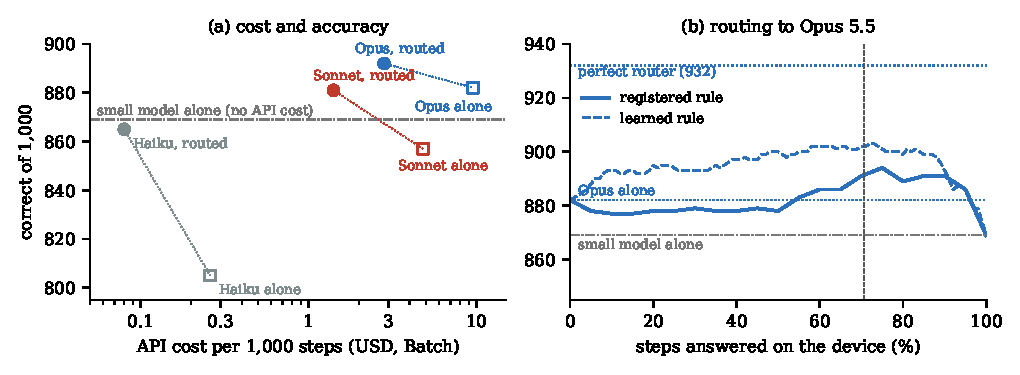
\includegraphics[width=0.56\linewidth]{fig_router.pdf}
\caption{Accuracy of the routed system as the share of locally answered steps varies (run 1). Dotted lines: frontier models alone. The gain appears once the small model keeps more than about half of the steps.}\label{fig:router}
\end{figure}

\paragraph{What stays local.} Table~\ref{tab:types} breaks run 1 down by action. The small model keeps nearly all scrolls down, waits, back presses, typing and app launches, and 59\% of taps. On the steps it keeps, its advantage over Opus comes mostly from the dataset's conventions, which Opus misapplies although its prompt states them and its examples show them (Table~\ref{tab:examples}): waiting when the previous action has not yet taken effect (50 vs 46), naming scroll direction by where new content appears (98 vs 92) and going back (33 vs 31), against 337 vs 334 on taps. Opus is slightly better on the kept typing and app-launch steps. The deferred steps are mostly taps, often on icons without text, which a text-only model cannot read.

\begin{table}[t]\centering\small
\caption{Run 1 by recorded action: share answered locally and correct answers on kept and deferred steps.}\label{tab:types}
\begin{tabular}{lrrccc}\toprule
Action & Steps & Kept & Small model, kept & Opus, kept & Opus, deferred\\\midrule
Tap & 605 & 59\% & 337/358 & 334/358 & 194/247\\
Scroll down & 102 & 96\% & 98/98 & 92/98 & 4/4\\
Type text & 88 & 93\% & 79/82 & 80/82 & 1/6\\
Open app & 79 & 99\% & 71/78 & 76/78 & 0/1\\
Wait & 62 & 81\% & 50/50 & 46/50 & 10/12\\
Back & 40 & 82\% & 33/33 & 31/33 & 6/7\\
Other scrolls & 24 & 33\% & 3/8 & 2/8 & 6/16\\\bottomrule
\end{tabular}\end{table}

\begin{table}[t]\centering\small
\caption{Examples from the held-out steps (instructions verbatim; confidence in parentheses).}\label{tab:examples}
\begin{tabular}{p{0.40\linewidth}p{0.15\linewidth}p{0.17\linewidth}p{0.16\linewidth}}\toprule
Instruction and history & Recorded action & Small model & Opus FS\\\midrule
``Click on the convert button''; same instruction as the previous step, screen half unchanged & wait & wait, kept (0.997) & tap\\
``Scroll up on the screen until you find the ratings \& reviews section'' & scroll down & scroll down, kept (0.996) & wait\\
``Click on the headphone icon to listen to news'' & tap the icon & deferred (0.635) & tap the icon\\\bottomrule
\end{tabular}\end{table}

\paragraph{Unseen apps, corrected labels and other scores.} These analyses were not registered. On the 457 steps from apps absent from training, routing to Opus scores 408 (89.3\%) against 405 (88.6\%) for Opus alone, and routing to Sonnet 403 (88.2\%) against 391 (85.6\%) for Sonnet alone. On AndroidControl-Curated labels~\citep{accurated} (995 matched steps), routing to Opus scores 928 (93.3\%) against 925 (93.0\%) for Opus alone ($+0.3$, $[-0.8, +1.4]$); routing to Sonnet scores 914 (91.9\%), $-1.1$ ($[-2.5, +0.3]$) against Opus alone, narrowly outside the margin. Over all 8{,}377 matched test steps the small model scores 92.0\% on curated labels and 88.6\% on the original ones. Ordering steps by the margin between the top two probabilities or by entropy gives the same accuracy as the registered score (890 and 889 with Opus at 70\% local); the action-type probability alone is clearly worse (862).

\paragraph{A learned deferral rule.} The registered score ignores how sure the model is about copied text, whether the chosen element is an icon without text, and the kind of action. We fit two logistic regressions on the separate sample used to set $\tau$, one predicting whether the small model is right and one whether few-shot Opus is right, from the action-type probability, margin and entropy, the element probability and margin, the copy-span probability, an unlabelled-icon flag, the predicted action type and the screen size (input length and element count). With standardised features $\phi(x)$, the rule scores each step by the predicted advantage
\[ \Delta(x) = \sigma\big(w_s^\top \phi(x)\big) - \sigma\big(w_f^\top \phi(x)\big) \]
and answers locally when $\Delta(x)$ exceeds a threshold; the weights are in Appendix~\ref{app:router}. Keeping the 70.7\% of steps with the largest $\Delta$, and testing on the held-out steps, routing to Opus scores 902 (run 1) and 900 (run 2) against 882 and 879 for Opus alone: $+2.0$ ($[+0.6, +3.4]$, $p=0.006$) and $+2.1$ ($[+0.8, +3.4]$, $p=0.003$), significantly better rather than only non-inferior; these steps were the rule's development set, so the confirmatory test below is the clean test. Routing to Sonnet scores 891 and 898. Against the registered rule the learned rule gains 0.9--1.0 points in all four comparisons, each not significant on its own ($p=0.10$--$0.14$). The learned rule changes which steps are deferred rather than how many: it sends every app launch and about a quarter of typing steps to Opus, which knows app names and copies text slightly better, and in exchange keeps 73\% of taps local instead of 59\% (back presses: 97\% instead of 82\%). We then froze this rule (weights and threshold) and registered a confirmatory test on 650 steps from 247 test episodes used in no earlier sample (the three test samples share no episodes; 10 of the 1{,}543 test episodes remain unused). There, routing to Opus with the learned rule scored 599 of 650 (92.2\%) against 581 (89.4\%) for Opus alone ($+2.8$ points, $[+1.0, +4.5]$; 26 steps gained, 8 lost; $p=0.003$; registered superiority supported) with 73.7\% of steps local; the registered threshold rule scored 595 (91.5\%; $+2.2$, $[+0.5, +3.9]$, $p=0.02$), and the two rules did not differ significantly ($+0.6$, $p=0.48$). The finding is therefore that routing beats Opus alone on fresh steps; the learned rule adds a point that we cannot separate from chance. Here the small model alone ties Opus (581 each), so the whole gain comes from the two models being right on different steps and the rule sending each step to the one more likely to be right, not from the small model being better. A perfect router would score 614, of which the learned rule recovers 55\%. On corrected labels (644 matched steps, not registered) the gain holds: the learned rule scores 613 against 593 for Opus ($+3.1$, $[+1.5, +4.7]$, $p<0.001$) and the registered rule 608 ($+2.3$, $[+0.7, +4.0]$, $p=0.008$). On the held-out sample the corresponding curated gains are smaller ($+0.3$ and $+1.0$, neither significant).

\paragraph{Pooled estimate.} The three test samples differ: the small model against Opus alone is $-1.5$, $-1.3$ and $0.0$ points on the calibration, held-out and confirmatory samples, and the routing gain on curated labels is $+0.3$ on the held-out and $+2.3$ on the confirmatory sample, a sample-to-sample spread of about 2 points. Pooling the 1{,}650 steps on which no routing choice was made (held-out and confirmatory), the registered rule beats Opus alone by $+1.5$ points ($[+0.5, +2.4]$; 47 steps gained, 23 lost; $p=0.006$) on original labels and by $+1.1$ ($[+0.2, +2.0]$, $p=0.03$, 1{,}639 matched steps) on curated labels, while the small model alone is $-0.8$ ($[-2.4, +0.8]$). The learned rule's pooled gains are $+2.3$ and $+1.8$, but its threshold was set on the held-out sample. The pooled registered-rule figure is the single number we would quote (\texttt{bench/ac\_pooled.py}).

\section{Clean Retrain and Fair Baselines}\label{sec:fair}
\paragraph{A clean retrain.} The small model's design was chosen while comparing variants on the test split. To rule out that this inflated the results, we retrained the same recipe with a new seed on 95\% of the training episodes, held out the remaining 5\% as a validation set, set the threshold on validation only (30th percentile, $\tau=0.9886$), and touched the test split once, for the final evaluation. A second retrain also removed empty, inert layout containers from the input (Sec.~\ref{sec:device}). On all 8{,}444 test steps the clean models score 88.1\% and 88.5\% against 88.5\% for the original (on the 122 test steps that the data labels as the unseen-app split, a narrower set than the apps absent from training used in Sec.~\ref{sec:router}: 88.5\% and 90.2\%, a difference of two steps that is not significant). Routing to Opus with the validation threshold (for the pruned model $\tau=0.9862$, from its whole validation set; Sec.~\ref{sec:sl} sets a separate threshold on half of it) is non-inferior to Opus alone on all three samples: $+1.1$, $+0.8$ and $+1.5$ points for the clean model and $+0.5$, $+0.8$ and $+1.2$ for the pruned one, with lower bounds of $-0.5$ or above; none of these differences is significant on its own ($p=0.08$--$0.44$).

\paragraph{The small model alone against frontier models.} 
\begin{table}[t]\centering\small
\caption{The separate sample of 1{,}000 test steps used to set $\tau$. ZS: no examples. Unseen apps: 401 steps.}\label{tab:frontier}
\begin{tabular}{llrrr}\toprule
System & Reasoning effort & Correct & Unseen apps & Cost (\$/1k)\\\midrule
Haiku 5.5 FS & low & 797 & -- & 0.25\\
Opus 5.5 ZS & low & 800 & 320 & 5.93\\
Sonnet 5.5 ZS & low & 804 & -- & 3.00\\
Opus 5.5 ZS & medium & 814 & -- & 6.08\\
Fable 5.1 FS & medium & 870 & 350 & 23.36\\
Small model & -- & 878 & 350 & 0\\
Opus 5.5 FS & medium & \textbf{893} & \textbf{359} & 9.44\\\bottomrule
\end{tabular}\end{table}

Without examples, Opus~5.5 and Sonnet~5.5 trail the small model by 7.8 and 7.4 points (both $p<10^{-5}$; Table~\ref{tab:frontier}, Fig.~\ref{fig:ac}). Many of their errors are dataset conventions rather than reasoning: 28 ``scroll down'' instructions answered with scroll up and 27 wait steps answered with a tap. At equal reasoning effort, 16 retrieved examples raise Opus from 814 to 893 ($+7.9$\pts, $p<10^{-14}$); on apps absent from training, Opus with examples scores 359 of 401 against 320 zero-shot at low effort. The small model is then 1.5 points behind Opus ($p=0.17$, CI $[-3.5, +0.5]$) and 0.8 ahead of Fable~5.1 ($p=0.52$). Fable's lower score is not a parsing failure (one unparsed reply in 1{,}000, on identical inputs): it wrote 29\% fewer output tokens than Opus and made more of the same convention errors (26 vs 16 missed waits, 8 vs 4 missed back presses), and it costs more only because of its price; the registered criterion, that it exceed every few-shot arm, is not met. For reference, on the full test set (8{,}444 steps) the small model scores 89.8\% in-domain and 86.7--87.9\% on the unseen-app, -task and -category splits, against 76.8--83.2\% for the best fine-tuned PaLM~2S~\citep{androidcontrol}; on a stricter holdout of 72 apps never seen in training it drops from 86.2\% to 82.6\%. Screenshot agents report AndroidControl-Low results under a more lenient protocol (a tap counts if it lands within 14\% of the screen width of the target, text if token F1 exceeds 0.5). Re-scored that way, on 7{,}868 test steps without waits and long presses (their set has 7{,}708), the small model scores 86.1\% (Table~\ref{tab:low}). This is below its strict accuracy on the same steps (88.3\%) because the protocol scores the centre of the chosen element as the tap point: on 312 taps the chosen element contains the recorded tap but its centre lies more than 14\% of the screen width away (wide list rows and tiles), against 106 taps and 28 text entries that only the protocol accepts. The result is above OS-Atlas-7B and below UI-TARS and InfiGUI-R1, from text alone and with 13--47 times fewer parameters. The step sets differ slightly, so the comparison is indicative.

\begin{table}[t]\centering\small
\caption{AndroidControl-Low step success under the OS-Atlas protocol. Other rows as reported by their authors; our step set differs slightly.}\label{tab:low}
\begin{tabular}{llrr}\toprule
Model & Input & Parameters & Step success (\%)\\\midrule
OS-Atlas-4B~\citep{osatlas} & screenshot & 4B & 80.6\\
OS-Atlas-7B~\citep{osatlas} & screenshot & 7B & 85.2\\
\textbf{Small model (ours)} & accessibility tree & 149M & \textbf{86.1}\\
UI-TARS-2B~\citep{uitars} & screenshot & 2B & 89.3\\
UI-TARS-7B~\citep{uitars} & screenshot & 7B & 90.8\\
InfiGUI-R1-3B~\citep{infiguir1} & screenshot & 3B & 92.1\\\bottomrule
\end{tabular}\end{table}

\begin{figure}[t]\centering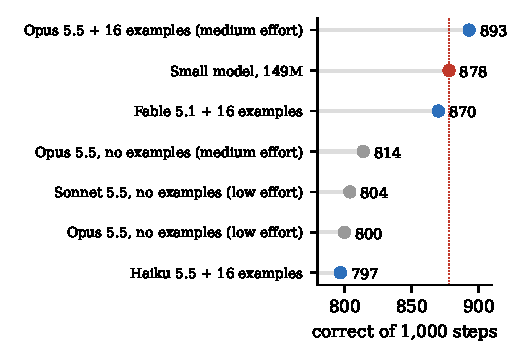
\includegraphics[width=0.5\linewidth]{fig_ac.pdf}
\caption{The sample used to set $\tau$. Grey: frontier models without examples. Blue: with 16 retrieved examples. Red: the small model.}\label{fig:ac}
\end{figure}

\section{A Fallback That Sees Only the Candidates}\label{sec:sl}
\paragraph{Deferred steps still carry local information.} When the small model defers a tap, its ranking of elements remains useful (not registered; no frontier calls). On the 247 deferred taps of the held-out steps its top-ranked element is right for 178 (72.1\%, against 194 for Opus), and the target is among its top 3 for 218 (88.3\%) and its top 5 for 225 (91.1\%). Of the 53 deferred taps that Opus gets wrong, the target is in the small model's top 5 for 45. On the 650 confirmatory steps the figures are 140 of 156 deferred taps in the top 5 (89.7\%) and 24 of the 32 Opus errors. A fallback that shows the frontier model the small model's top candidates, rather than the whole screen, could therefore recover many of the remaining errors and shorten its input. The registered test below asks whether it does.

\paragraph{Registered test.} All but 10 test episodes had been used, so this registered test (AC-Shortlist) draws 1{,}000 fresh steps from the validation episodes of the clean pruned-input retrain, which it never trained on. These episodes come from the training split, so apps and task templates overlap with training: the test is in-domain. The threshold ($\tau=0.9842$) was set on the other half of the validation episodes; 746 steps stay local and 254 are deferred. Three fallback inputs were compared on the deferred steps: the full screen; the full screen plus the numbers of the small model's top 5 elements; and only those 5 elements, with the rest of the screen kept on the device. The registered fallback was Opus; to limit API cost, an amendment committed before any frontier call replaced it with Haiku~5.5 and added Sonnet~5.5 with the full screen as a secondary comparison. Table~\ref{tab:sl} gives the results. Showing only the candidates is non-inferior to showing the full screen ($+0.7$, $[-0.5, +1.9]$; 185 against 178 of the deferred steps), halves the fallback's input (2{,}463 against 4{,}983 tokens per call, including the examples) and sends 5 elements per deferred screen off the device instead of the whole screen. The hint alongside the full screen did not help significantly ($+0.5$, $[-0.6, +1.6]$, $p=0.47$). The registered comparison with Sonnet, Haiku with the hint against Sonnet with the full screen, missed non-inferiority narrowly ($-0.8$, $[-2.1, +0.5]$, margin 2). Haiku shown only the candidates came closer ($-0.6$, $[-1.9, +0.7]$), at about a thirtieth of Sonnet's fallback cost, but that comparison was not registered. On these in-domain steps the small model alone already scores 90.3\%, and no routed system is significantly better than it ($-0.2$ to $+1.1$, $p\ge0.21$); the fallback matters most where the small model is weaker, as on the test split. With Haiku, a fallback no better than the small model on these steps (178 against 180 deferred steps right), the test shows that the candidates lose nothing, not that they recover errors. The decisive test, with Opus on the strict 72-app holdout where the small model is weaker, is future work.

\begin{table}[t]\centering\small
\caption{AC-Shortlist: 1{,}000 fresh in-domain steps; 746 answered locally, 254 deferred. Costs are billed Batch API costs for the deferred steps (Haiku alone: all 1{,}000 steps).}\label{tab:sl}
\begin{tabular}{lrrr}\toprule
System & Deferred correct (of 254) & Overall (\%) & Cost (USD)\\\midrule
Small model alone & 180 & 90.3 & 0\\
Haiku~5.5 alone, full screen & -- & 82.6 & 0.27\\
Routed, Haiku, full screen & 178 & 90.1 & $\approx$0.07\\
Routed, Haiku, full screen + top-5 hint & 183 & 90.6 & 0.08\\
Routed, Haiku, top-5 elements only & 185 & 90.8 & 0.04\\
Routed, Sonnet~5.5, full screen & 191 & 91.4 & 1.35\\\bottomrule
\end{tabular}\end{table}


\section{Running on a Phone}\label{sec:device}
We exported the model to ONNX and ran it with ONNX Runtime~1.20 on the CPU of a Pixel~6a (4 threads) over 40 real inputs (median 1{,}228 tokens). At full precision the outputs match PyTorch on all 40 steps, with a median latency of 4.5\,s (90th percentile 11.9\,s) and 1.94\,GB peak memory. With 8-bit weights (150\,MB on disk) latency falls to 3.4\,s (11.2\,s) and memory to 1.45\,GB. Over all 1{,}000 held-out steps the 8-bit model scores 851 alone (869 at full precision), keeps 66.6\% of steps under the unchanged threshold, and routing still holds: 886 against 882 for Opus alone ($+0.4$, $[-0.7, +1.5]$). Most of this loss comes from sharing one scale per weight tensor. Choosing on the calibration sample among three quantization settings, we picked per-channel scales (151\,MB, same size); on the held-out steps it scores 862 alone, recovering 11 of the 18 lost steps, and agrees with full precision on 975 of 1{,}000 outcomes (885 against 882 routed to Opus). The phone latencies in this section were measured with the per-tensor model; on a laptop CPU the two run at the same speed. On a laptop GPU (Apple M2, fp16) the median is 0.29\,s. Most of the input is layout containers that show nothing and cannot be acted on. Removing them before encoding cuts the median input from 1{,}247 to 800 tokens on the held-out steps; without retraining this costs 0.8 points (861 vs 869), and a model retrained on pruned input loses nothing (88.5\% on the full test split). Routing stays intact (888 against 882 for Opus alone; 879 against 857 for Sonnet alone; 71.3\% local). On the phone, the 8-bit model with pruned input takes a median 1.18\,s (90th percentile 4.9\,s), 2.9 times faster than unpruned, because attention cost grows faster than input length. Peak memory stays at 1.45\,GB, dominated by ONNX Runtime's memory pool rather than by activations: disabling the pool lowers it to 0.97\,GB but doubles latency. Sub-second latency on the phone will need its neural accelerator or a smaller encoder.

As a demonstration, with the model on a laptop driving the phone over USB, the small model completed a five-step Clock task (open the Timers tab, enter 5:00, start the timer) from step instructions, answering every step locally in 0.22--0.31\,s.

\section{Live Multi-Step Tasks}\label{sec:live}
Offline evaluation starts every step from the recorded history, so errors cannot compound. On AndroidWorld~\citep{androidworld} (116 live tasks) a related cascade, in which a goal-only variant of the small model acted when confident and otherwise the T3A agent with Gemini-3.5-Flash acted, completed fewer tasks than T3A alone (41.9\% vs 54.8\%, $p=0.008$, 93 tasks valid in both arms); a registered variant with app-name grounding and a no-effect guard also trailed (50.4\% vs 58.3\%). Run-to-run variation is large: across 43 identically configured episodes with greedy decoding, 65\% followed a different action sequence and 9\% changed outcome. A second registered design split the work the other way: a frontier planner wrote one to five step instructions from a compressed screen and the small model executed them, re-planning on low confidence or an unchanged screen. In an offline pilot on goal-only AndroidControl steps it scored 49.0\% against 61.3\% for the planner's model acting alone, with 5.6 times fewer frontier tokens. Taps were close (65.4\% vs 69.1\%); the loss came from the planner's instructions for app launches, waits and scrolls, which did not follow the conventions the small model had learned; the next step is to train the planner to write instructions in those conventions, distilled from the training episodes, and to repeat the live test. Jev-Mobile~\citep{jevmobile} reports a similar split on AndroidWorld (79\% vs 84\% at 73\% lower cost) with a remote decision service as the executor rather than an on-device model. The offline results above should not be read as evidence for deployed multi-step agents.

\section{Discussion and Limitations}
\paragraph{What the evidence supports.} For single steps with a step instruction, a 149M model can take about 70\% of a phone agent's steps while the routed system stays within 2 points of a frontier model that sees the same training data, at 15--30\% of its cost. The result replicates, holds on unseen apps and, for Opus, on corrected labels, and survives 8-bit quantization. On a further registered sample, routing is significantly more accurate than Opus alone with either rule; on corrected labels (not registered) the gain holds, and pooled over both test samples it is $+1.5$ points. Most of the benefit is nevertheless cost and data exposure: seven in ten screens never leave the device. The fallback must be strong; Haiku behind the small model does not help on the test split (865 against 869 for the small model alone). With Haiku as the fallback on in-domain steps, showing it only the small model's five best elements lost nothing against the full screen at half the input; whether the candidates help a strong fallback on unseen apps is untested.

\paragraph{What it does not support.} The small model alone is not better than a frontier model given the same examples, and its advantage on the steps it keeps comes from AndroidControl's labelling conventions (waiting, scroll direction), not from better grounding. Without step instructions the picture is mixed: in an earlier registered study on 1{,}000 fresh goal-only steps, a goal-only variant of the small model with Gemini-3.5-Flash as fallback scored 67.0\% against 58.0\% for Flash with eight fixed examples ($+9.0$, $[+6.3, +11.8]$), calling Flash on 38\% of steps, but that baseline was weaker than the retrieved-example baseline used here, and the same design lost live (Sec.~\ref{sec:live}). The model is too slow on a phone CPU for interactive use.

\paragraph{Limitations.} Inputs are text only, so unlabelled icons are hard. The original model's design was selected using the AndroidControl test split during development; clean retrains that never used the test split for any choice reach the same accuracy (Sec.~\ref{sec:fair}). Both the small model and the frontier prompts rely on 74{,}714 labelled in-domain steps. The frontier models were given text only; a screenshot could help them most on the deferred steps, many of which are taps on unlabelled icons, so a multimodal frontier baseline may be stronger than ours; we leave that comparison to future work. The headline small model is a single training seed; a second seed under the clean protocol scored 88.1\% against 88.5\%, and three seeds on an 18{,}481-step training subset gave $80.8\pm0.7$\%. The frontier models are proprietary API versions that may change. Costs exclude on-device compute and the latency of a second call. Phone measurements cover one device and one runtime. This paper draws on a log of about 40 registered experiments and amendments, many with negative outcomes (Table~\ref{tab:neg}); each result reported here was confirmed on data not used to design it, but we apply no correction across the program.

\begin{table}[t]\centering\small
\caption{Hypotheses not supported and ideas that did not help.}\label{tab:neg}
\begin{tabular}{p{0.52\linewidth}p{0.4\linewidth}}\toprule
Hypothesis or idea & Outcome\\\midrule
Small model better than few-shot frontier models & Not supported (878 vs 893 for Opus, $p=0.17$)\\
No accuracy drop on apps unseen in training & Not supported on a 72-app holdout ($-3.6$\pts)\\
Cascade to Haiku~4.5, then Sonnet (AndroidControl) & 842, below the small model alone\\
Routing to Haiku~5.5 matches Opus & Not supported ($-1.7$ $[-3.5, +0.1]$)\\
Live cascade, distillation, self-training, completion guard & Below the frontier agent or no change\\
Retrieval memory for the small model; ModernBERT-large & $+0.0$ to $+0.3$\pts; 81.7\% vs 88.5\%\\\bottomrule
\end{tabular}\end{table}

\section*{Broader Impact}
A phone agent acts for a person and can expose what is on the screen. Keeping most steps local reduces what reaches a cloud provider but does not remove it: 29.3\% of screens were still sent. Automated actions can cause harm (purchases, messages, deletions), and we did not evaluate safeguards. The live demonstration used an app that requires no account, and no personal data was recorded. AndroidControl is released under the Apache~2.0 license.

\section*{Reproducibility}
We release the registration log with its commit history, the evaluation harness and prompts, the per-step outputs and billed token counts of every frontier request, the routing and re-scoring scripts, the trained model (safetensors and ONNX) with a one-call Python interface, the phone benchmark and the demonstration script. Tables~\ref{tab:router}--\ref{tab:types} and the routing curves are recomputed by one script from the released files without new model calls, and a test suite asserts them; the curated-label, unseen-app and latency analyses also need the AndroidControl text file (built by a released notebook) or a phone.

\section*{Use of AI Assistance}
The author designed and directed this work. Code, analyses and drafting were done with substantial help from Claude (Anthropic), and independent AI reviews were used to check the analysis and presentation. The author is responsible for the content.

\bibliography{refs}
\bibliographystyle{tmlr}

\appendix
\section{Training Details}\label{app:train}
ModernBERT-base fine-tuned for 2 epochs on the 74{,}714 AndroidControl training steps with AdamW (learning rate $5\times10^{-5}$, weight decay 0.01), batch size 1 with 8-step gradient accumulation, 200 warm-up steps and linear decay, fp16 mixed precision, on one NVIDIA T4 GPU, seed 0. Inputs are truncated to 28 tokens per element and 3{,}072 tokens in total. Losses: cross-entropy over action types; for taps, a multi-positive cross-entropy over element markers in which every element whose centre lies inside the target counts as correct; for typed text and app names, cross-entropy over start and end positions (weight 0.5).

\paragraph{Extraction versus generation (preliminary).} In a registered comparison at equal training data (18{,}481 steps), on test steps that fit the generators' context, the encoder with copy heads was 2.4--6.8 points more accurate than LoRA-tuned Qwen2.5-3B and 7B models that generate the action as text; three encoder seeds gave $80.8\pm0.7\%$ on that subset. The generators' inputs were truncated from the front on long screens during training, and the 7B scored below the 3B, so we treat this as preliminary and draw no conclusion from it.

\section{Learned Deferral Rule}\label{app:router}
Both logistic regressions were fit on the sample used to set $\tau$ (1{,}000 steps) with L2 penalty 1 by gradient descent on standardised features; the threshold on $\Delta$ ($-0.0101$) keeps 70.7\% of the routing sample local. Table~\ref{tab:weights} lists the frozen weights; the released file holds the means and standard deviations.

\begin{table}[!htbp]\centering\small
\caption{Frozen weights on standardised features. $w_s$: small model correct; $w_f$: few-shot Opus correct. A positive difference favours answering locally.}\label{tab:weights}
\begin{tabular}{lrrr}\toprule
Feature & $w_s$ & $w_f$ & $w_s - w_f$\\\midrule
Intercept & 2.28 & 2.31 & $-0.03$\\
log action-type probability & 0.01 & $-0.11$ & 0.12\\
Action-type margin & $-0.30$ & $-0.28$ & $-0.02$\\
Action-type entropy & $-0.94$ & $-0.63$ & $-0.32$\\
log element probability (taps) & 0.30 & $-0.08$ & 0.38\\
Element margin (taps) & 0.31 & 0.50 & $-0.20$\\
log copy-span probability & 0.07 & 0.06 & 0.01\\
Chosen element has no text & $-0.23$ & $-0.16$ & $-0.07$\\
log input length & 0.12 & 0.21 & $-0.09$\\
log element count & $-0.31$ & $-0.18$ & $-0.13$\\
Predicted tap or long press & 0.08 & 0.09 & $-0.02$\\
Predicted type text & 0.00 & 0.00 & 0.01\\
Predicted open app & $-0.21$ & 0.15 & $-0.36$\\
Predicted wait & $-0.23$ & $-0.29$ & 0.06\\
Predicted back or home & 0.22 & 0.02 & 0.20\\
Predicted scroll & 0.09 & $-0.02$ & 0.11\\\bottomrule
\end{tabular}\end{table}

\section{Registered Experiments}\label{app:reg}
\begin{table}[!htbp]\centering\small
\caption{Registrations this paper relies on; all entries, with timestamps and amendments, are in the released log.}\label{tab:reg}
\begin{tabular}{p{0.22\linewidth}p{0.44\linewidth}p{0.26\linewidth}}\toprule
Registration & Question & Outcome\\\midrule
AC, AC-Opus & Small model vs zero-shot frontier models; three-tier cascade & Small model ahead; cascade 842\\
AC-Fair (+ effort control) & Small model vs few-shot Opus~5.5 and Fable~5.1 & Not better; examples add 7.9\pts\\
AC-Router & Routing to few-shot Opus on held-out steps & Non-inferior; 70.7\% local\\
AC-Router-Sonnet & Routing to few-shot Sonnet & Non-inferior to Sonnet and Opus\\
AC-Router-Rerun & Second run of Opus and Sonnet & Replicated\\
AC-Router-Haiku & Routing to few-shot Haiku & Non-inferior to Haiku only\\
AC-LearnedRouter & Frozen learned rule vs Opus alone, 650 new steps & Better than Opus ($+2.8$, $p=0.003$)\\
AC-Shortlist (+ amendment) & Fallback sees only the small model's top 5 elements & Non-inferior to full screen; hint alone no gain\\
W3--W12 & A separate web system (not reported here) & See log\\
E14b--E14d & Goal-only routing offline (Gemini 3.5 Flash / Pro) & Routing $+9.0$ over few-shot Flash\\
E13--E24 (live) & Live cascades, distillation, self-training, guards & Below frontier agent or null\\
E1, E4, E5 & Copying vs generating; seeds; generator scale & Copying ahead of 3B/7B generators by 2.4--6.8\pts; 3 seeds $80.8\pm0.7$\%\\
E2 & Goal-only small model vs LiMAC (63.1\%) & Not supported: 61.7\% [60.5, 63.0]\\
E3, E6--E12 & Model scale, features, selective prediction & Design choices; see log\\\bottomrule
\end{tabular}\end{table}
\end{document}
